%%%%%%%%%%%%%%%%%%%%%%%%%%%%%%%%%%%%%%%%%%%%%%%%%%%%%%%%%%%%%%%%%%%%%%%%%%%%%%%%
%2345678901234567890123456789012345678901234567890123456789012345678901234567890
%        1         2         3         4         5         6         7         8

\documentclass[letterpaper, 10 pt, conference]{ieeeconf}  % Comment this line out if you need a4paper
%\graphicspath{{../../Thesis/assets/}}
%\documentclass[a4paper, 10pt, conference]{ieeeconf}      % Use this line for a4 paper

\IEEEoverridecommandlockouts                              % This command is only needed if 
                                                          % you want to use the \thanks command

\overrideIEEEmargins                                      % Needed to meet printer requirements.

% See the \addtolength command later in the file to balance the column lengths
% on the last page of the document

% The following packages can be found on http:\\www.ctan.org
\usepackage{graphicx} % for pdf, bitmapped graphics files
\usepackage{epsfig} % for postscript graphics files
%\usepackage{mathptmx} % assumes new font selection scheme installed
%\usepackage{times} % assumes new font selection scheme installed
%\usepackage{amsmath} % assumes amsmath package installed
%\usepackage{amssymb}  % assumes amsmath package installed
\usepackage{epstopdf}

\usepackage{hyperref}
\usepackage{subcaption}
\usepackage[linesnumbered,ruled,vlined]{algorithm2e}

\title{\LARGE \bf
Indriya : A platform for designing human robot interaction scenarios based on human behaviors
}


\author{Praveenkumar Vasudevan$^{1}$ and Gentiane Venture$^{2}$% <-this % stops a space
\thanks{*This work was supported by JASSO}% <-this % stops a space
\thanks{$^{1}$Praveenkumar Vasudevan is a graduate student in robotics at Ecole centrale de Nantes,
        1 rue de la noe, 44000 Nantes, France
        {\tt\small praveenv4k@gmail.com}}%
\thanks{$^{2}$Gentiane Venture is an Associate Professor at the Department of Mechanical Systems Engineering, Tokyo University of Agriculture and Technology,
        2-24-16 Koganei, Tokyo - 1848588, Japan
        {\tt\small venture@cc.tuat.ac.jp}}%
}


\begin{document}



\maketitle
\thispagestyle{empty}
\pagestyle{empty}


%%%%%%%%%%%%%%%%%%%%%%%%%%%%%%%%%%%%%%%%%%%%%%%%%%%%%%%%%%%%%%%%%%%%%%%%%%%%%%%%
\begin{abstract}

In scenarios where robots coexist with humans in a social environment, understanding both verbal and non-verbal communication is extremely inevitable. Together they convey information such as intention, emotion and even health of a human, that adds value to the way robots participate in an interaction. On the other hand, the people who design interaction scenarios are from diverse fields who do not essentially have the required robot programming skills. In this paper a new behavior programming paradigm and an easy to use visual programming interface for the same is proposed, which gives the power to design human-robot interaction taking into account human behaviors. The distributed platform namely Indriya proposed in this paper gives the ability to plug and play multimodal sensors and diverse class of robots. The platform usage has been demonstrated using scenarios where NAO robot performs actions understanding human behavior using Microsoft Kinect sensor. %Finally the platform is validated using statistical analysis performed on the user study conducted on a set of participants.

\end{abstract}


%%%%%%%%%%%%%%%%%%%%%%%%%%%%%%%%%%%%%%%%%%%%%%%%%%%%%%%%%%%%%%%%%%%%%%%%%%%%%%%%
\section{INTRODUCTION}

The richness and diversity of Human Robot Interaction (HRI) has been described in \cite{dautenhahn2007methodology} as ``HRI is a challenging research field at the intersection of psychology, cognitive science, social sciences, artificial intelligence, computer science, robotics, engineering and human-computer interaction". Goodrich in his extensive survey \cite{goodrich2007human} proposed two main types of HRI namely remote interaction and proximate interaction. The latter has led to the development of a new class of robots called social robots. Yan et al. \cite{yan2014survey} define ``A social robot is a robot which can execute designated tasks and the necessary condition turning a robot into a social robot is the ability to interact with humans by adhering to certain social cues and rules.''

	Social robots already entered the human spaces as entertainers, educators, caring agents and personal assistants \cite{Aldebaran}. Hence the design and the development of interaction systems need to be approached in a systematic manner wherein the robots should be able to understand the human behaviors in order to interact in a better way. To make it possible it is necessary to develop robotic systems with essential perceptual ability for efficient and natural interaction. Most often the on-board sensors on the robots fail to satisfy this demanding requirement due to various constraints like space, power and computational needs. Therefore consideration of augmenting exteroceptive sensors that are commonly available in the smart home/public environments to this purpose is essential.

	Another important aspect is that the HRI designers are from diverse backgrounds. People study various aspects such as robot ethics, social acceptance, liveliness, cultural influence etc., from various perspectives like sociology, psychology, humanities and so on. So the tools needed to design behaviors of a social robot should be intuitive and user friendly.  With increased availability of social robots and cost effective human activity recognition sensors, we could still observe a huge void which inhibits the exploitation of available technology for designing robot behaviors for human-in-the-loop scenarios.

	The main contribution of this paper are: \textbf{(a)} A distributed and modular \textit{Application framework} which gives opportunity to interface multimodal sensor systems and diverse class of robots. \textbf{(b)} A simple and easy to understand \textit{Behavior program model} in order to design reactive human robot interaction scenarios. \textbf{(c)} An intuitive and easy to use \textit{User interface} to design, execute and monitor interaction from broad range of client devices. 

 The paper is organized as follows. Section~\ref{sec:related_work} discusses the state-of-the-art techniques. Section~\ref{sec:indriya_platform} presents a brief introduction to Indriya architecture. Section~\ref{sec:system_evaluation} describes the system capabilities and Section~\ref{sec:user_study} presents the user study results.  Finally Section~\ref{sec:conclusion} presents the concluding remarks.

\section{RELATED WORK}
\label{sec:related_work}
Human behavior understanding can be broadly classified into non-verbal/motion recognition and verbal/speech recognition. Vision based motion capture and analysis systems have been one of the first class citizens in the human motion analysis which is summarized in surveys \cite{moeslund2006survey}\cite{poppe2007vision}. Vision based human pose estimation has traditionally suffered from the requirement to adopt an initialization pose and losing track after a few frames. These problems have been addressed in \cite{shotton2013efficient} which proposes methods to track accurately the human skeletons using single depth images. Understanding of human motion is not complete if the action of the human could not be inferred. In the survey \cite{han2013enhanced}, a study on various algorithms used for human activity analysis is presented. Recently data-driven machine learning approaches have proven to be successful with recognition accuracy as high as 94.9\% \cite{Kinect2014}. The verbal communication instead has been studied by human computer interaction community for many years now  \cite{reddy1976speech} \cite{lippmann1997speech} and led to the development of software toolkits that implements state-of-the-art algorithms \cite{SpeechSdk}.
	
	The localization of humanoid robots is a challenging issue, due to rough odometry estimation, noisy onboard sensing, and the swaying motion caused by walking \cite{cervera2012localization}. Studies on robot localization, obstacle mapping, and path planning by equipping NAO with a consumer-level depth camera have been reported in \cite{maier2012real}. Localization and motion planning in smart home environment using an external kinect sensor have been proposed in \cite{cervera2012localization}. These methods are computationally demanding and it could cause overall performance degradation particularly when one wants to share the same sensor for both human motion recognition and localization of the robot. Tracking rectangular fiducial markers using augmented reality tool-kits like ALVAR \cite{ALVAR} can be interesting if one could embed those markers on the humanoid robot. This is one of the simplest and cheapest solutions in terms of computational power as it can provide position and orientation of the physical markers in real time.
	
	The users of social robots do not have necessarily backgrounds in programming and design of robot behaviors. The main challenge in the behavior design is the ability to define the behavior which can abstract complex data flows from the end user. There exists flow-chart based visual programming languages \cite{Choregraphe} which allow non-programmers to create robot applications using a set of pre-built behavioral blocks. These programs are very intuitive but when it comes to designing reactive behaviors for human-in-the-loop scenarios, the existing visual programming methods increase the cognitive load on the end users. Specialized robot programming techniques like Task description language \cite{simmons1998task} and middlewares like ROS \cite{quigley2009ros} have been proposed in the literature. Though these systems provide modular and distributed architecture, support multiple sensors and robots etc., these require high level of skill in robotics and programming. Recently non-domain-specific solution like Targets-Drives-Means is proposed in \cite{berenz2014targets}, however it lacks an intuitive interface.
\section{INDRIYA PLATFORM}
\label{sec:indriya_platform}
We propose a platform namely ``Indriya'', for designing human robot interaction scenarios taking inspiration from distributed architecture \cite{quigley2009ros} and intuitive visual programming techniques \cite{Blockly}. 
\subsection{System Architecture}
The system setup and architecture are shown in Fig~\ref{fig:indriya}. The principal components of the architecture are
\begin{figure}[thpb]
\centering
\begin{subfigure}[t]{0.48\columnwidth}
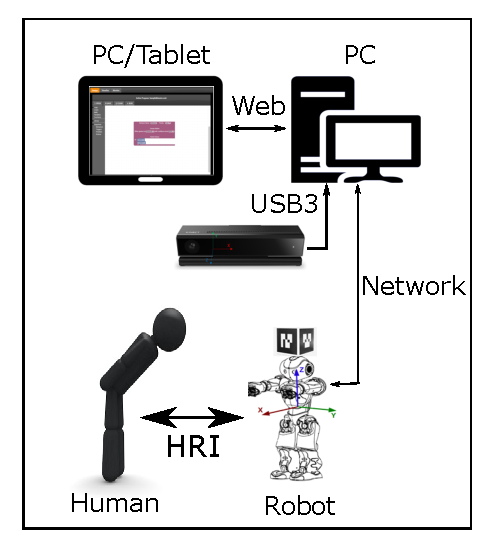
\includegraphics[width=\columnwidth]{../../thesis/assets/system_setup.eps}
\caption[System setup]{System setup}
\label{fig:setup}
\end{subfigure}
\begin{subfigure}[t]{0.48\columnwidth}
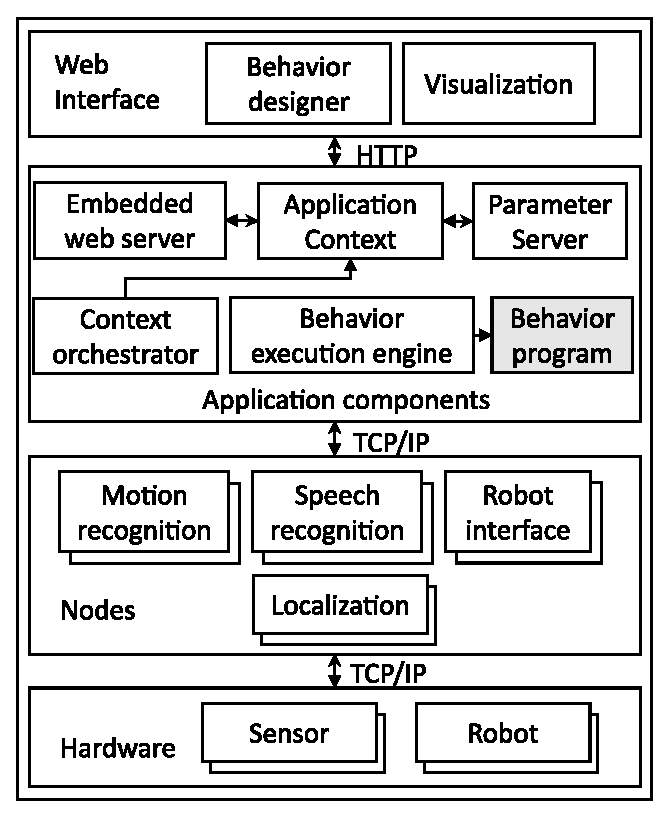
\includegraphics[width=\columnwidth]{../../thesis/assets/indriya_architecture.eps}
\caption[Software architecture]{Software architecture}
\label{fig:architecture}
\end{subfigure}
\caption[Indriya Platform]{Indriya Platform}
\label{fig:indriya}
\end{figure}
\subsubsection{Hardware layer} : It is composed of robots and sensors which are connected to the Indriya application server. 
\subsubsection{Distributed Layer} : It is composed nodes each with a specific goal that can run in any machine inside the network. All the nodes will communicate with the application using message passing techniques. The most important nodes in the system are: 
\emph{Motion Recognition Node} that interacts with a motion recognition sensor and sends the detected motions and gestures to the application. Additionally each motion recognition module registers a set of motions/gestures that could be detected with the sensor associated with it, \emph{Speech Recognition Node} that makes use of the pre-configured grammar file for language of interest to recognize the human speech, \emph{Robot Interface Node} that interacts with a specific robot and can invoke a set of actions on it. It also sends periodic update about the robot status to the application. Moreover it registers a set of parameterizable actions that could be invoked on the robot associated with it.\emph{Localization Node} that uses the perception system to compute the position and orientation of the robot and humans in the environment.
\subsubsection{Application Components}
The \emph{Application context} contains the complete description of the world. It contains latest information about all the robots and humans in the environment. The \emph{Parameter Server} acts as a central repository for managing the parameters of the system. The \emph{Embedded Web Server} is responsible for data and file transaction between the Indriya system and the web client through a set of RESTful services. The \emph{Context Orchestrator} keeps the application context uptodate by synchronizing with information  published by the distributed components.
\subsubsection{User Interface}: The user interface is a web application that runs on any latest web-kit browsers supporting WebGL technology. The prime goal of this UI is to make it suitable for environments adopting bring your own device (BYOD) policy. The UI is composed of: A \emph{Behavior Designer} that could be used by the user to drag and drop the behavior blocks and construct the program by putting together motion recognition blocks and robot action blocks. The designer offers a full range of capabilities like Create/Edit/Delete/Save behavior programs. The \emph{Visualization} could be used to see the interaction of the human and robot inside a virtual 3D environment.
\subsection{Behavior Program}
\label{ssec:behavior_program}
\begin{figure}
\centering
\begin{subfigure}[t]{0.48\columnwidth}
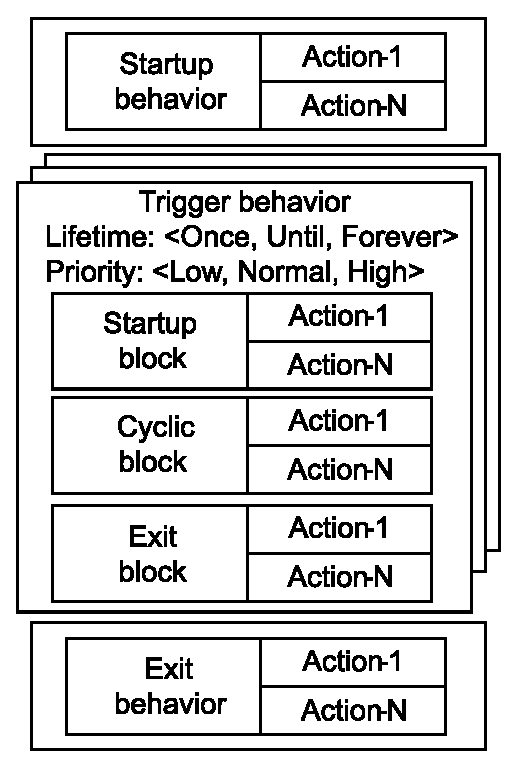
\includegraphics[width=\columnwidth]{../../thesis/assets/program_structure.eps}
\caption[Conceptual Model]{Conceptual Model}
\label{fig:program_concept}
\end{subfigure}
\begin{subfigure}[t]{0.48\columnwidth}
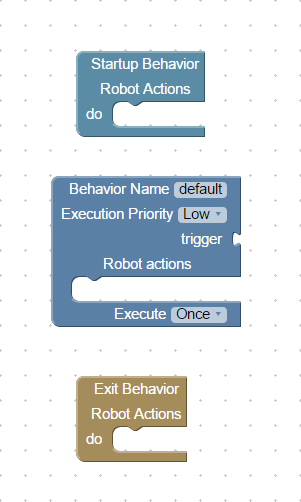
\includegraphics[width=\columnwidth]{../../thesis/assets/behavior_blocks.png}
\caption[Block Implementation]{Block Implementation}
\label{fig:program_blocks}
\end{subfigure}
\caption[Program Structure]{Behavior program structure}
\label{fig:program}
\end{figure}
The behavior program is structured in a simple way so that it could be easily understood by the end user. The conceptual model of behavior program is shown in Fig.~\ref{fig:program_concept} and the block level implementation is shown in Fig.~\ref{fig:program_blocks}. The behavior program is composed of:

\emph{Startup and Exit behavior}: The start-up behavior will be executed once when the user starts the program. The user can add a set of actions to be performed when the program starts. Similarly the exit block will be executed once when the lifetime of all the configured behavior blocks expire.  Both these blocks are optional and there cannot be more than one instances of these in a program.

\emph{Trigger behavior}: The behavior block is the core component of the behavior program. The block could be activated by the interaction between the human and the robot. There could be many behavior blocks in a program.
\begin{table}[h]
\caption{Trigger behavior properties}
\label{trigger_behavior}
\begin{center}
\begin{tabular}{|c|c|}
\hline
  \textbf{Property} & \textbf{Description}\\
\hline
Trigger & Block activation trigger.\\
{}		& Gesture/speech trigger, vicinity of human etc.,\\
\hline
Lifetime & Behavior lifetime. \\
{}       & Once, Forever or Until a condition is met\\
\hline
Priority & Behavior priority. \\
{}       & Uses fixed priority premptive scheduling\\
\hline
\end{tabular}
\end{center}
\end{table}
\subsection{Code generation and execution}
Each of the visual behavior program blocks has an associated code generation module and C\# code is generated from the blocks from the blocks. Traditionally there is a need to compile the C\# code and generate binaries when one wants to execute it. Thanks to the latest compiler technologies and tools like ScriptCS \cite{ScriptCS}, it is now possible to run the C\# code like scripts. This is exploited in the Indriya platform.
\begin{figure}
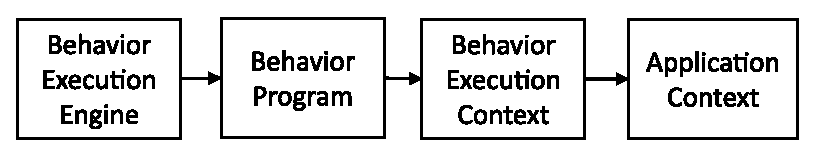
\includegraphics[width=\columnwidth]{../../thesis/assets/execution_flow.eps}
\caption[Behavior program - Execution flow]{Behavior program - Execution flow}
\label{fig:program_execution}
\end{figure}

\begin{algorithm}
 \KwData{program : Behavior program}
 startup := STARTUP\_BEHAVIORS(program)\;
 exit := EXIT\_BEHAVIORS(program)\;
 triggered := TRIGGER\_BEHAVIORS(program)\;
 sorted := SORT\_PRIORITY(triggered)\;
 \If{startup}{
  EXECUTE\_BEHAVIOR(startup)\;
 }
 \While{behavior lifetime}{
  \ForAll{behavior in sorted}{
    \If{behavior not complete}{
      \If{CHECK\_TRIGGER(behavior)}{
        current = GET\_ACTIVE\_TASK()\;
        priority1 = PRIORITY(behavior)\;
        priority2 = PRIORITY(current)\;  
        \If{priority1 $>$ priority2}{
          DO\_PREMEPTION(current)\;
          SCHEDULE\_TASK(behavior)\;
        }
        \ElseIf{no active task}{
          SCHEDULE\_TASK(behavior)\;
        }
      }
    }
  }
 }
 \If{exit}{
  EXECUTE\_BEHAVIOR(exit)\;
 }
 \caption{Behavior execution algorithm}
 \label{alg:behavior_engine}
\end{algorithm}
 The execution flow of the behavior program is shown in Fig.~\ref{fig:program_execution}. The generated behavior program is consumed by a \emph{Behavior execution engine} which dynamically identifies the configured behavior blocks. The main functionality of the behavior execution engine is to check if the trigger condition of the behavior blocks is met and once the condition is met, the execution of the corresponding behavior is scheduled on a separate CPU thread. The behavior program accesses the uptodate information about the environment through an interface namely the \emph{Behavior execution context} which acts as a proxy to the \emph{Application context}. The algorithm of the behavior execution by the engine is shown in Algorithm~\ref{alg:behavior_engine}.
\section{IMPLEMENTATION}
The platform is implemented using open network communication standards equipped by ZeroMQ library \cite{ZeroMQ} and message serialization is done using Google protocol buffers \cite{ProtocolBuffers}. The node information and parameters of nodes are configured using an XML file. A set of human motion clips are captured and gesture recognizer is trained using the Visual gesture builder tool that comes with Microsoft Kinect SDK. Similarly a set of commonly used speech commands are configured in the grammar files to be used by the speech recognition node. The localization of the robot is achieved using a marker cube mounted on the head of the humanoid robot. ALVAR \cite{ALVAR} marker tracking library is used along with a 2-DOF kinematic model from torso to the tip of the head of the robot.  A set of actions are developed for NAO humanoid robot such as approaching a human, saying expressively etc., and corresponding visual blocks are also developed. The software is tested on a 64-bit Intel Core i7 CPU with clock speed 3.60 Ghz and 8 GB of RAM on a Microsoft Windows 8.1 OS. The source code of the software is available as open source at \url{https://github.com/praveenv4k/Indriya}
\section{SYSTEM EVALUATION}
\label{sec:system_evaluation}
In this section various capabilities of Indriya platform are evaluated
\subsection{Intuitiveness}
\textbf{Scenario:} The NAO humanoid robot is a guide in a museum. The museum manager would like to design a scenario where when a visitor comes into the vicinity of the robot, the robot would approach him/her and start explaining the history of the museum. The experiment setup for this scenario is shown in Fig~\ref{fig:scenario1_setup}.

\begin{figure}
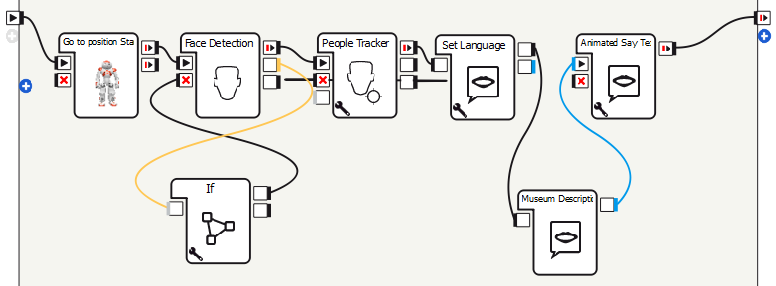
\includegraphics[width=\columnwidth]{../../thesis/assets/scenario_museum_choregraphe3.png}
\caption[NAO museum guide: Choregraphe program]{NAO museum guide: Choregraphe program}
\label{fig:scenario1_program_choregraphe}
\end{figure}
\begin{figure}
\centering
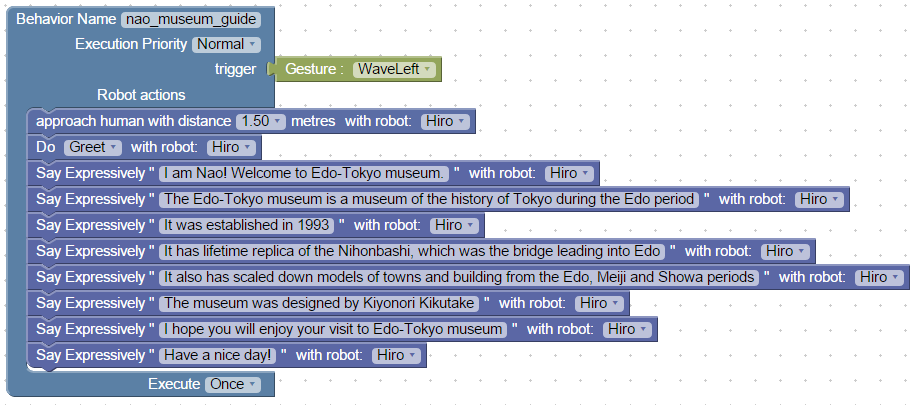
\includegraphics[width=\columnwidth]{../../thesis/assets/scenario1_new.png}
\caption[NAO museum guide: Indriya program]{NAO museum guide: Indriya program}
\label{fig:scenario1_program}
\end{figure}
 We would like to use this scenario to compare the simplicity and straight forwardness of behavior description with Choregraphe \cite{Choregraphe} shown in Fig~\ref{fig:scenario1_program_choregraphe} and with our interface shown in Fig~\ref{fig:scenario1_program}. Though Choregraphe uses a familiar flow-chart based programming model and has a huge library of primitive blocks to build complex motion patterns, the data flow for this scenario is not straight forward. As could be noticed from Fig~\ref{fig:scenario1_program_choregraphe}, at first the robot keeps looking for people in its vicinity using the \emph{Face detection block} at the cost of its power. Once it detects a person, the face detection block is stopped and \emph{People tracker} block is activated. The robot starts approaching (tracking) the person until a fixed distance with the person is reached. Once the desired distance of separation is achieved, the people tracker block is stopped. Now the robot will actually start explaining the history of the museum. For a novice programmer it could be difficult to think of this dataflow as they literally have to emulate the whole scenario in their mind before designing the system.

The Indriya platform equipped with Kinect sensor takes care of the detection of people and gives the relative localization of the robot and human. Once the person is detected or a configured gesture trigger arrives, the behavior program retrieves the relative transformation of the robot with respect to human. The \emph{Approach block} makes use of this information to drive the robot towards the person. After coming into the proximity of the person, the robot starts explaining the history of museum. From the user perspective, the design of the behavior is \emph{intuitive} using Indriya. He/She can focus on the scenario rather than thinking about the minute details of the data flow. 

\subsection{Realistic scenarios}
\textbf{Scenario:} A physiotherapist who is in a remote hospital would like to prepare an exercise routine for his patient who is recovering from the fracture of his left hand. The therapist wants the service robot in the rehabilitation center to give directions to the patient in an interactive manner and facilitate the process. The exercise is composed of: an introduction and demonstration of the routine, interactively reporting the progress of the exercise and finally notifying the completion. The experiment setup is shown in Fig.~\ref{fig:scenario2_setup}

\begin{figure}
\begin{subfigure}[t]{0.48\columnwidth}
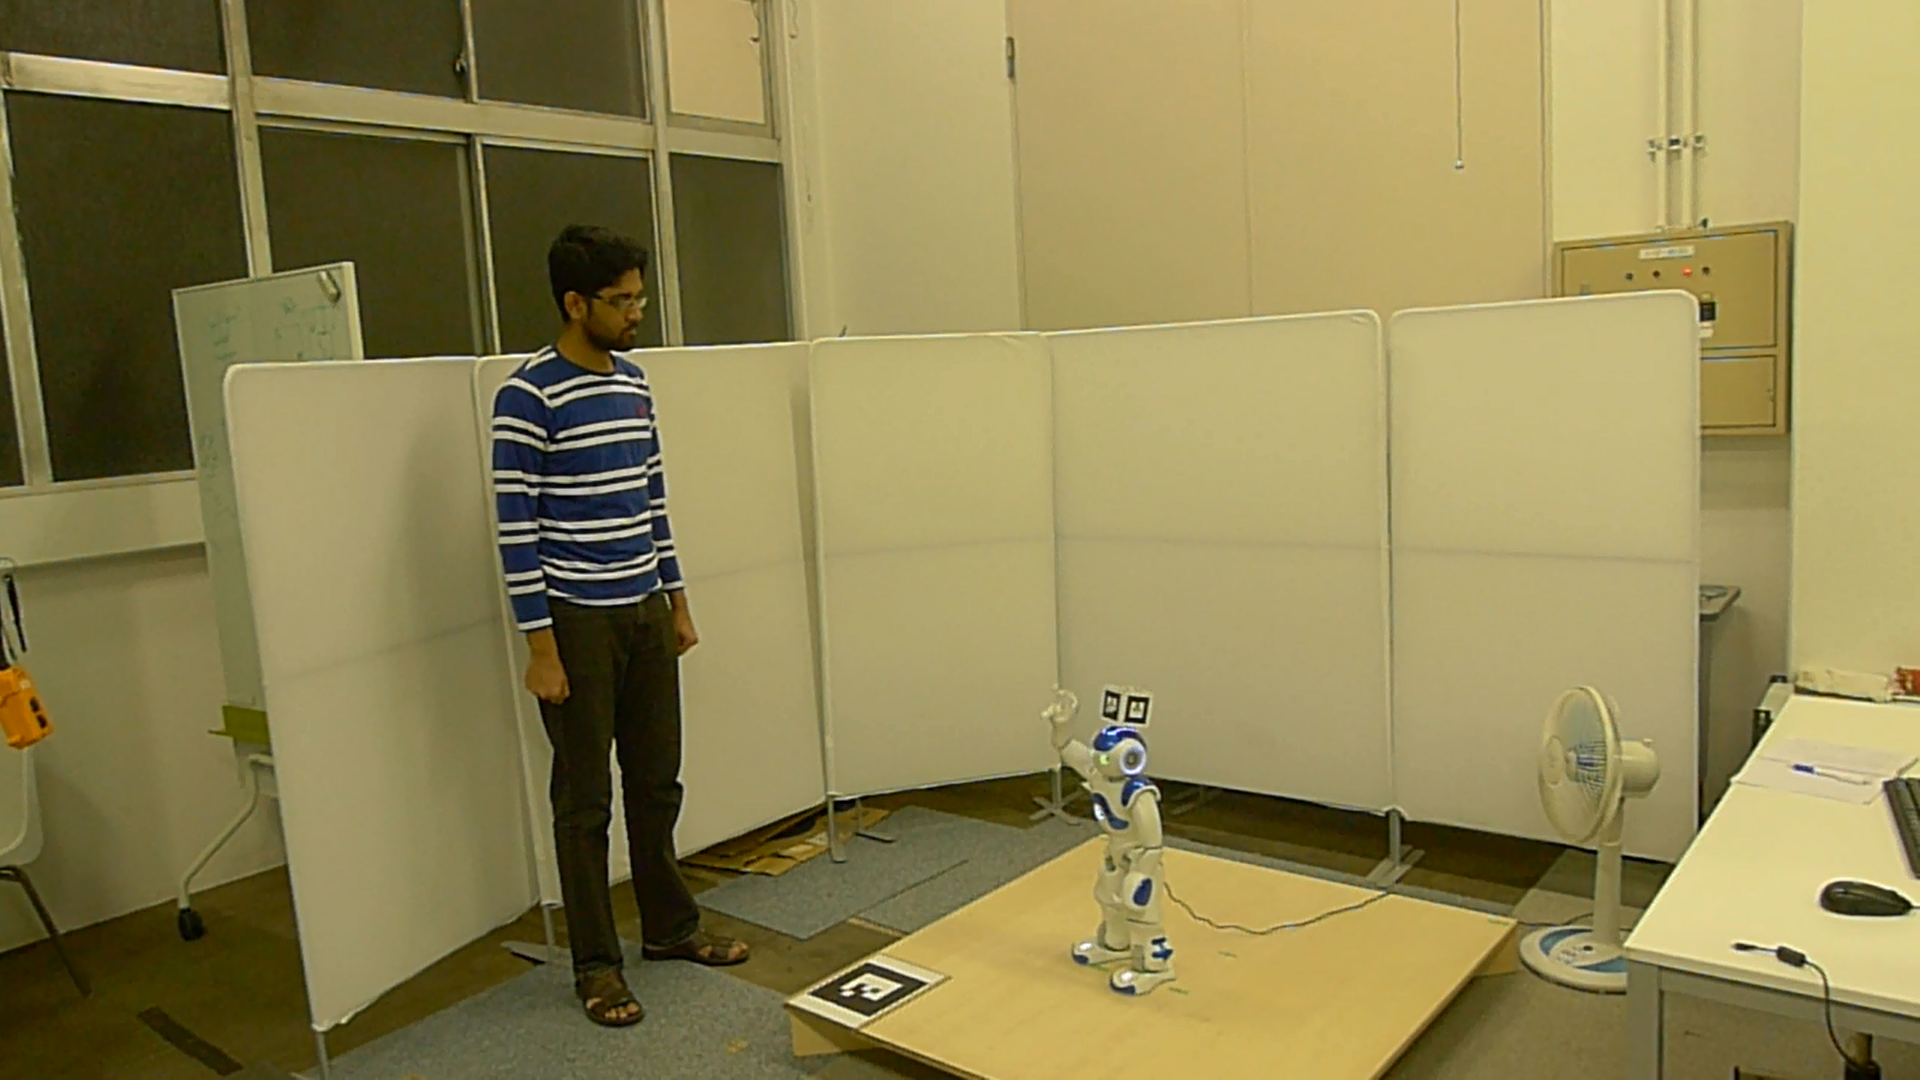
\includegraphics[width=\columnwidth]{../../thesis/assets/scenario_museum.png}
\caption[NAO museum guide: Experiment setup]{NAO museum guide}
\label{fig:scenario1_setup}
\end{subfigure}
\begin{subfigure}[t]{0.48\columnwidth}
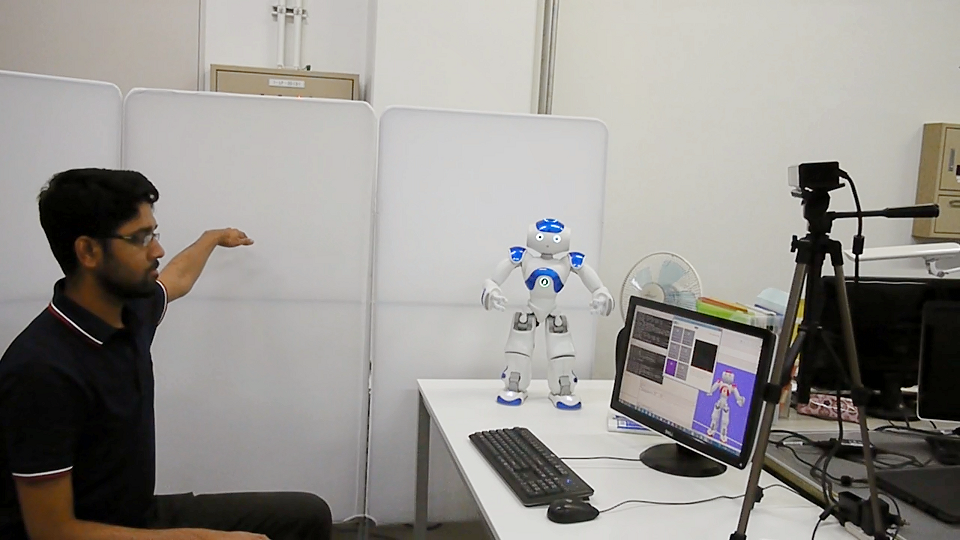
\includegraphics[width=\columnwidth]{../../thesis/assets/scenario_therapy.png}
\caption[NAO therapy facilitator: Experiment setup]{NAO therapy facilitator}
\label{fig:scenario2_setup}
\end{subfigure}
\caption[Experiment setup]{Experiment setup}
\label{fig:experiment_setup}
\end{figure}
Though Choregraphe software gives the capability of programming behaviors with basic human awareness, it does not explicitly allows programming that takes into account human gestures/motions. This is not the drawback of the system but the fact that it does not have enough sensors to understand complex motions. Thanks to the Kinect sensor and its gesture recognition capabilites, one can exploit it to design a program for the above scenario using our platform as shown in Fig~\ref{fig:scenario2_program}.

\begin{figure}
\centering
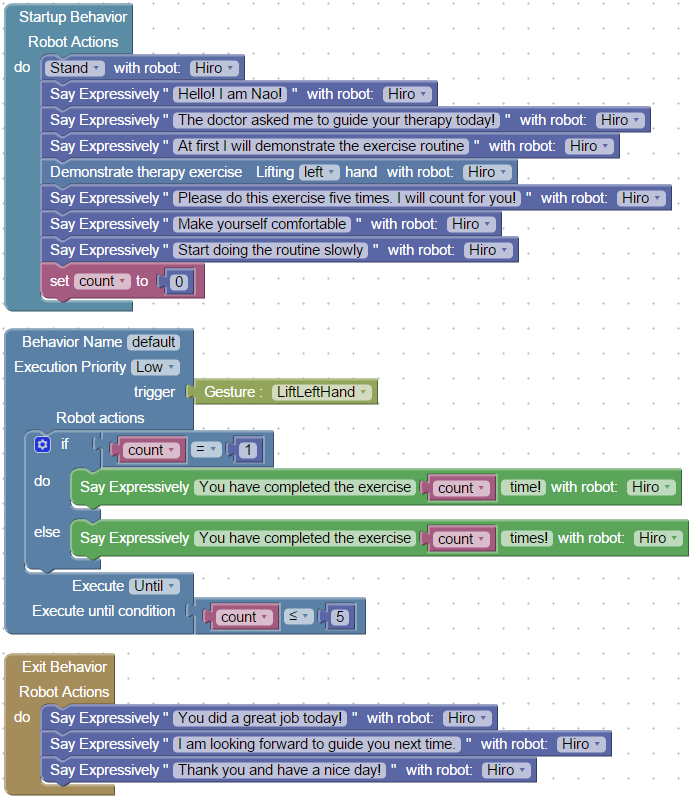
\includegraphics[width=\columnwidth]{../../thesis/assets/scenario2_new.png}
\caption[NAO therapy facilitator: Indriya program]{NAO therapy facilitator: Indriya program}
\label{fig:scenario2_program}
\end{figure}
The scenario is designed using all the three basic behavior constructs that constitutes the behavior program. In the startup behavior the robot gives an introduction about the exercise routine and then gives a demonstration of how to do it. A trigger behavior block is configured to be triggered each time when the patient performs the therapy routine (lifting left hand). Each time the patient performs the exercise a variable is incremented and the robot notifies the progress by announcing how many times the patient has completed the exercise. The trigger behavior block is configured \emph{Until} a desired condition on the exercise count is reached (say lifting left hand 5 times). Once the lifetime of the trigger behavior block expires, the robot gives some closing comments about the routine. It could be noticed that the description of this scenario is quite simple using Indriya. The blockly editor powered with the behavior program logic abstracts the complexity of designing realistic scenarios.

\subsection{Priority execution}
Most often in real life HRI scenarios one would like to have robot respond to certain events with a higher priority irrespective of what it is doing at that time. Priority based execution capability comes handy in such scenarios. The inherent problem is that often these concepts are extremely difficult to understand/implement for beginner to intermediate level programmers. The Indriya system makes this extremely easy by just fixing the priority of each behavior blocks. 

\textbf{Scenario:} Let us consider an elderly care robot who takes care of a fictitious person Mr. Adams. The living room is equipped with kinect sensor so that the activities and voice commands of the person could be recognized by Indriya system. The care taker of Mr. Adams who is working during the day would like to design a behavior program for the robot. He/She wants the robot to respond to normal commands like \emph{Come here}, \emph{Bring Coffee} etc., Among others he would like the robot to serve emergency conditions like when the elderly person faint down suddenly, or he/she asks for help due to medical complications etc.,

The reference implementation of the caring robot is shown in Fig.~

\subsection{Programming Multi-robots and Parallel tasks}
The Indriya system is designed in such a way that it is easy to create multiple instances of robot interface module targeted at a single robot type (say NAO) by just changing the connection parameters. The visual blocks are also designed so that it is easy to select the robot on which the task should be executed, by an user-defined name. Additionally the platform makes it simpler to execute parallel tasks on two or more robots without any hassles.

\textbf{Scenario:} Let us consider a product introduction event in which the product team decided to use robots to give an introduction and demonstration of their product. Let us assume that the robots say \emph{Hiro} and \emph{Taro} were used to give an introduction about \emph{Indriya} platform and its capabilities like multi-robot support, parallel execution, gesture/voice recognition support and priority based execution support etc., A reference implementation of this scenario is shown in Fig~\ref{fig:complex_parallel_program}

\begin{figure}
\centering
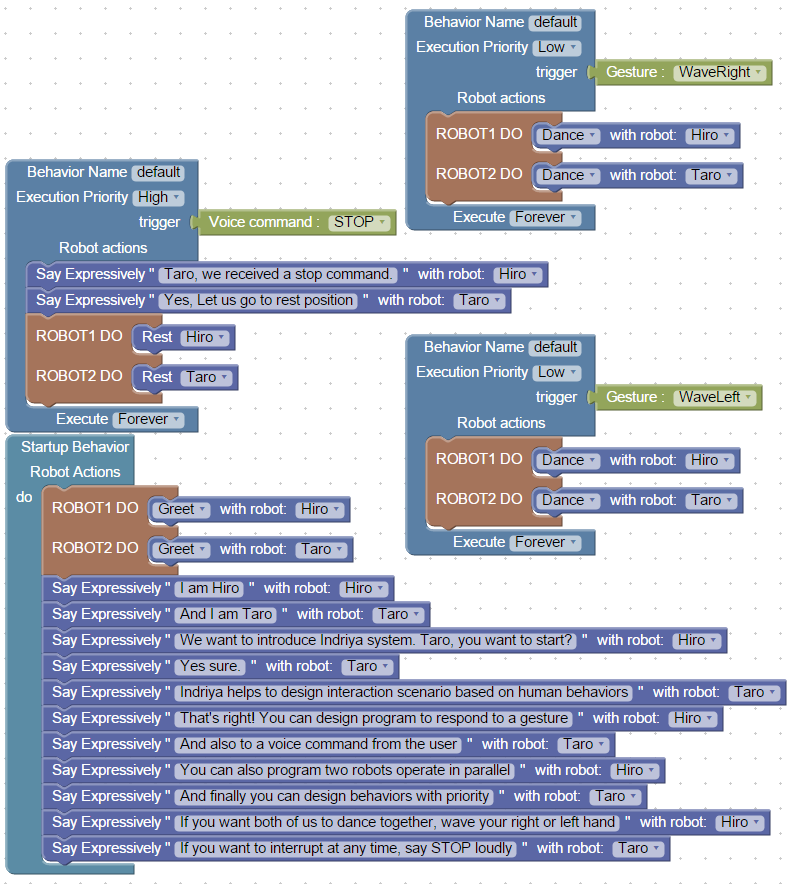
\includegraphics[width=\columnwidth]{../../thesis/assets/complex_parallel_scenario.png}
\caption[Product demo scenario: Indriya program]{Product demo scenario: Indriya program}
\label{fig:complex_parallel_program}
\end{figure}
Even for an intermediate programmer implementing such a scenario using say a system like ROS \cite{quigley2009ros} will be a daunting job. Parallel programming using multiple threads is tricky at times. Depending on the OS and programming language used, the constructs to build programs for parallel execution of tasks is difficult. With robots it is even more difficult job as the execution has to be monitored while serving other high priority human triggers. The Indriya platform gives a breezy user interface with which all these problems are effectively addressed.
\section{USER STUDY}
\label{sec:user_study}
\subsection{Protocol}
The interaction design process suggested in \cite{Rogers2011} has been followed. The participants were given a short introduction about the system with the help of a handout describing the platform. The participants were given a maximum of 90 minutes to think, design and execute the scenario designed. They were given a maximum of 2 chances to edit and execute the scenario on the real robot. Irrespective of whether they manage to complete what they desired at the end of two chances, they were asked to evaluate the system based on their experience of using the platform. A questionnaire is prepared in both English and Japanese for the data collection purpose and the questionnaire is integrated in the user interface as shown in Fig.\ref{fig:ui_evaluate}. The questions are designed with a 4-point semantic differential scale.
 \begin{figure}
 \centering
 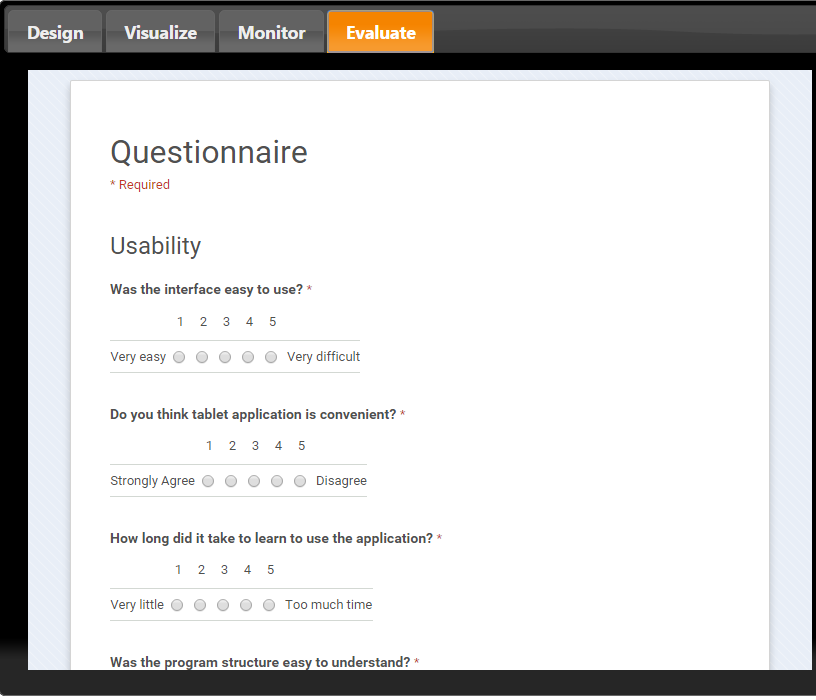
\includegraphics[width=0.8\columnwidth]{../../thesis/assets/questionnaire_integration.png}
 \caption[Questionnaire integration in UI]{Questionnaire integration in UI}
 \label{fig:ui_evaluate}
 \end{figure}
\subsection{Data analysis}
Statistical analysis is performed on the data collected during the user study. The usability metrics such as learnability, effectiveness, efficiency and satisfaction are measured. 
\subsection{Observations}
\section{CONCLUSIONS}
\label{sec:conclusion}
The abundance of smart devices and sensors in the smart home and public environments could be used for an immersive and personalized human robot interaction experience. However people from interdisciplinary fields find it difficult to use the existing technology as it requires strong background in programming. Any new programming paradigm designed for such purposes should find a correct balance between simplicity and expressiveness which motivated us to develop this platform. There exist some open questions and challenges to be addressed. The preliminary challenges are to find a set of all possible human activities that could be understood from the sensors distributed around in the environment and to identify all possible actions a robot could perform to interact with human in a social interaction scenario. The next question is to find the spectrum of interaction scenarios this kind of programming interface could cover. We believe these issue could be effectively addressed owing to the modular design and extensible nature of our platform.
\section{Prospective work}
\label{sec:prospects}
\quad This is a work in progress and for the moment we have evaluated our system for the Kinect system working seamlessly with the NAO humanoid robot for a set of predefined gestures/speech commands and robot actions. We are planning to develop an extensive database containing commonly encountered gestures and also an extensive set of primitive robot actions. Additionally we are also planning to integrate our system to work with other modes of motion recognition like inertial measurement units (IMU), accelerometers and gyroscopes that are available in smart-phones and wearable devices. Similarly we are planning to integrate our system with other robots like Pepper which we expect to receive soon.
\addtolength{\textheight}{-12cm}   % This command serves to balance the column lengths
                                  % on the last page of the document manually. It shortens
                                  % the textheight of the last page by a suitable amount.
                                  % This command does not take effect until the next page
                                  % so it should come on the page before the last. Make
                                  % sure that you do not shorten the textheight too much.

%%%%%%%%%%%%%%%%%%%%%%%%%%%%%%%%%%%%%%%%%%%%%%%%%%%%%%%%%%%%%%%%%%%%%%%%%%%%%%%%



%%%%%%%%%%%%%%%%%%%%%%%%%%%%%%%%%%%%%%%%%%%%%%%%%%%%%%%%%%%%%%%%%%%%%%%%%%%%%%%%



%%%%%%%%%%%%%%%%%%%%%%%%%%%%%%%%%%%%%%%%%%%%%%%%%%%%%%%%%%%%%%%%%%%%%%%%%%%%%%%%
\section*{ACKNOWLEDGMENT}

We would like to thank the members of GVLab at Tokyo University of Agriculture and Technology for helping us arranging the resources and participating in the experimentation.

%%%%%%%%%%%%%%%%%%%%%%%%%%%%%%%%%%%%%%%%%%%%%%%%%%%%%%%%%%%%%%%%%%%%%%%%%%%%%%%%

%\begin{thebibliography}{99}
%
%\bibitem{c1} G. O. Young, �Synthetic structure of industrial plastics (Book style with paper title and editor),� 	in Plastics, 2nd ed. vol. 3, J. Peters, Ed.  New York: McGraw-Hill, 1964, pp. 15�64.
%\bibitem{c2} W.-K. Chen, Linear Networks and Systems (Book style).	Belmont, CA: Wadsworth, 1993, pp. 123�135.
%\bibitem{c3} H. Poor, An Introduction to Signal Detection and Estimation.   New York: Springer-Verlag, 1985, ch. 4.
%\bibitem{c4} B. Smith, �An approach to graphs of linear forms (Unpublished work style),� unpublished.
%\bibitem{c5} E. H. Miller, �A note on reflector arrays (Periodical style�Accepted for publication),� IEEE Trans. Antennas Propagat., to be publised.
%\bibitem{c6} J. Wang, �Fundamentals of erbium-doped fiber amplifiers arrays (Periodical style�Submitted for publication),� IEEE J. Quantum Electron., submitted for publication.
%\bibitem{c7} C. J. Kaufman, Rocky Mountain Research Lab., Boulder, CO, private communication, May 1995.
%\bibitem{c8} Y. Yorozu, M. Hirano, K. Oka, and Y. Tagawa, �Electron spectroscopy studies on magneto-optical media and plastic substrate interfaces(Translation Journals style),� IEEE Transl. J. Magn.Jpn., vol. 2, Aug. 1987, pp. 740�741 [Dig. 9th Annu. Conf. Magnetics Japan, 1982, p. 301].
%\bibitem{c9} M. Young, The Techincal Writers Handbook.  Mill Valley, CA: University Science, 1989.
%\bibitem{c10} J. U. Duncombe, �Infrared navigation�Part I: An assessment of feasibility (Periodical style),� IEEE Trans. Electron Devices, vol. ED-11, pp. 34�39, Jan. 1959.
%\bibitem{c11} S. Chen, B. Mulgrew, and P. M. Grant, �A clustering technique for digital communications channel equalization using radial basis function networks,� IEEE Trans. Neural Networks, vol. 4, pp. 570�578, July 1993.
%\bibitem{c12} R. W. Lucky, �Automatic equalization for digital communication,� Bell Syst. Tech. J., vol. 44, no. 4, pp. 547�588, Apr. 1965.
%\bibitem{c13} S. P. Bingulac, �On the compatibility of adaptive controllers (Published Conference Proceedings style),� in Proc. 4th Annu. Allerton Conf. Circuits and Systems Theory, New York, 1994, pp. 8�16.
%\bibitem{c14} G. R. Faulhaber, �Design of service systems with priority reservation,� in Conf. Rec. 1995 IEEE Int. Conf. Communications, pp. 3�8.
%\bibitem{c15} W. D. Doyle, �Magnetization reversal in films with biaxial anisotropy,� in 1987 Proc. INTERMAG Conf., pp. 2.2-1�2.2-6.
%\bibitem{c16} G. W. Juette and L. E. Zeffanella, �Radio noise currents n short sections on bundle conductors (Presented Conference Paper style),� presented at the IEEE Summer power Meeting, Dallas, TX, June 22�27, 1990, Paper 90 SM 690-0 PWRS.
%\bibitem{c17} J. G. Kreifeldt, �An analysis of surface-detected EMG as an amplitude-modulated noise,� presented at the 1989 Int. Conf. Medicine and Biological Engineering, Chicago, IL.
%\bibitem{c18} J. Williams, �Narrow-band analyzer (Thesis or Dissertation style),� Ph.D. dissertation, Dept. Elect. Eng., Harvard Univ., Cambridge, MA, 1993. 
%\bibitem{c19} N. Kawasaki, �Parametric study of thermal and chemical nonequilibrium nozzle flow,� M.S. thesis, Dept. Electron. Eng., Osaka Univ., Osaka, Japan, 1993.
%\bibitem{c20} J. P. Wilkinson, �Nonlinear resonant circuit devices (Patent style),� U.S. Patent 3 624 12, July 16, 1990. 
%
%
%
%
%
%
%\end{thebibliography}

\bibliographystyle{IEEEtran}
\bibliography{IEEEabrv,biblio}
%\bibliographystyle{ieeetr} % Use the "unsrtnat" BibTeX style for formatting the Bibliography

%\bibliography{biblio}


\end{document}
